\documentclass[10pt]{article}
%\usepackage{wallpaper}
\usepackage[spanish]{babel}
\usepackage[utf8]{inputenc}
\usepackage[top=1in, bottom=1.0in, left=1.in, right=1.in]{geometry}

\usepackage{amsmath}
\usepackage{graphicx}
\usepackage{animate}
\usepackage{amssymb}
\usepackage{gensymb}
\usepackage[makeroom]{cancel}
\usepackage{mathtools}% Loads amsmath
\usepackage{tikz}
\usepackage{multicol}

\newcommand{\angstrom}{\text{\normalfont\AA}}
\newlength\myheight
\newcommand*\ccircled[1]{\settowidth{\myheight}{#1}%
    \raisebox{-.1\myheight}{\tikz[baseline=(char.base)]{%
        \node[shape=circle,draw,minimum size=1.5em,inner sep=1pt](char){#1};}}}
        
\pagestyle{empty}
\setlength\parindent{0pt}

\begin{document}

%\vspace{1.5cm}
%\hfill{Buenos Aires, \today} \\

\begin{center}
 {\large \bf Estructura Electrónica de Materias: \\
 Cálculo desde primeros principios} \\
 
\vspace{0.25cm}
 Guía Práctica N\degree 4
\end{center}

\vspace{0.5cm}
A. Resultados para Fe con estructura BBC y pseudopotenciales GGA:

\vspace{0.5cm}
(1) Caso magnético:
\begin{multicols}{2}
Convergencia en {\verb KPOINTS }:
\begin{verbatim}
K      Energía total 
4      -4.085001
6      -4.108849
8      -4.121582
10     -4.121930
12     -4.121572
\end{verbatim}

Convergencia en {\verb ENCUT }.
\begin{verbatim}
ENCUT  Energía total
300    -4.121582
350    -4.119746
400    -4.117555
450    -4.117370
500    -4.117559
\end{verbatim}
\end{multicols}
 

\vspace{0.5cm}
(2) Caso no magnético:

\begin{multicols}{2}
Convergencia en {\verb KPOINTS }:
\begin{verbatim}
K      Energía total 
4      -3.797970
6      -3.847494
8      -3.822858
10     -3.828644
12     -3.825857
14     -3.826873
\end{verbatim}

Convergencia en {\verb ENCUT }.
\begin{verbatim}
ENCUT  Energía total
300    -3.830041
350    -3.828032
400    -3.825857
450    -3.825617
500    -3.825819

\end{verbatim}
\end{multicols}


5. Para los casos estudiados anteriormente, la convergencia de 
la energía total a la variación del parámetro de red se muestra 
en la siguiente figura:
\begin{figure}[h]
\centering
 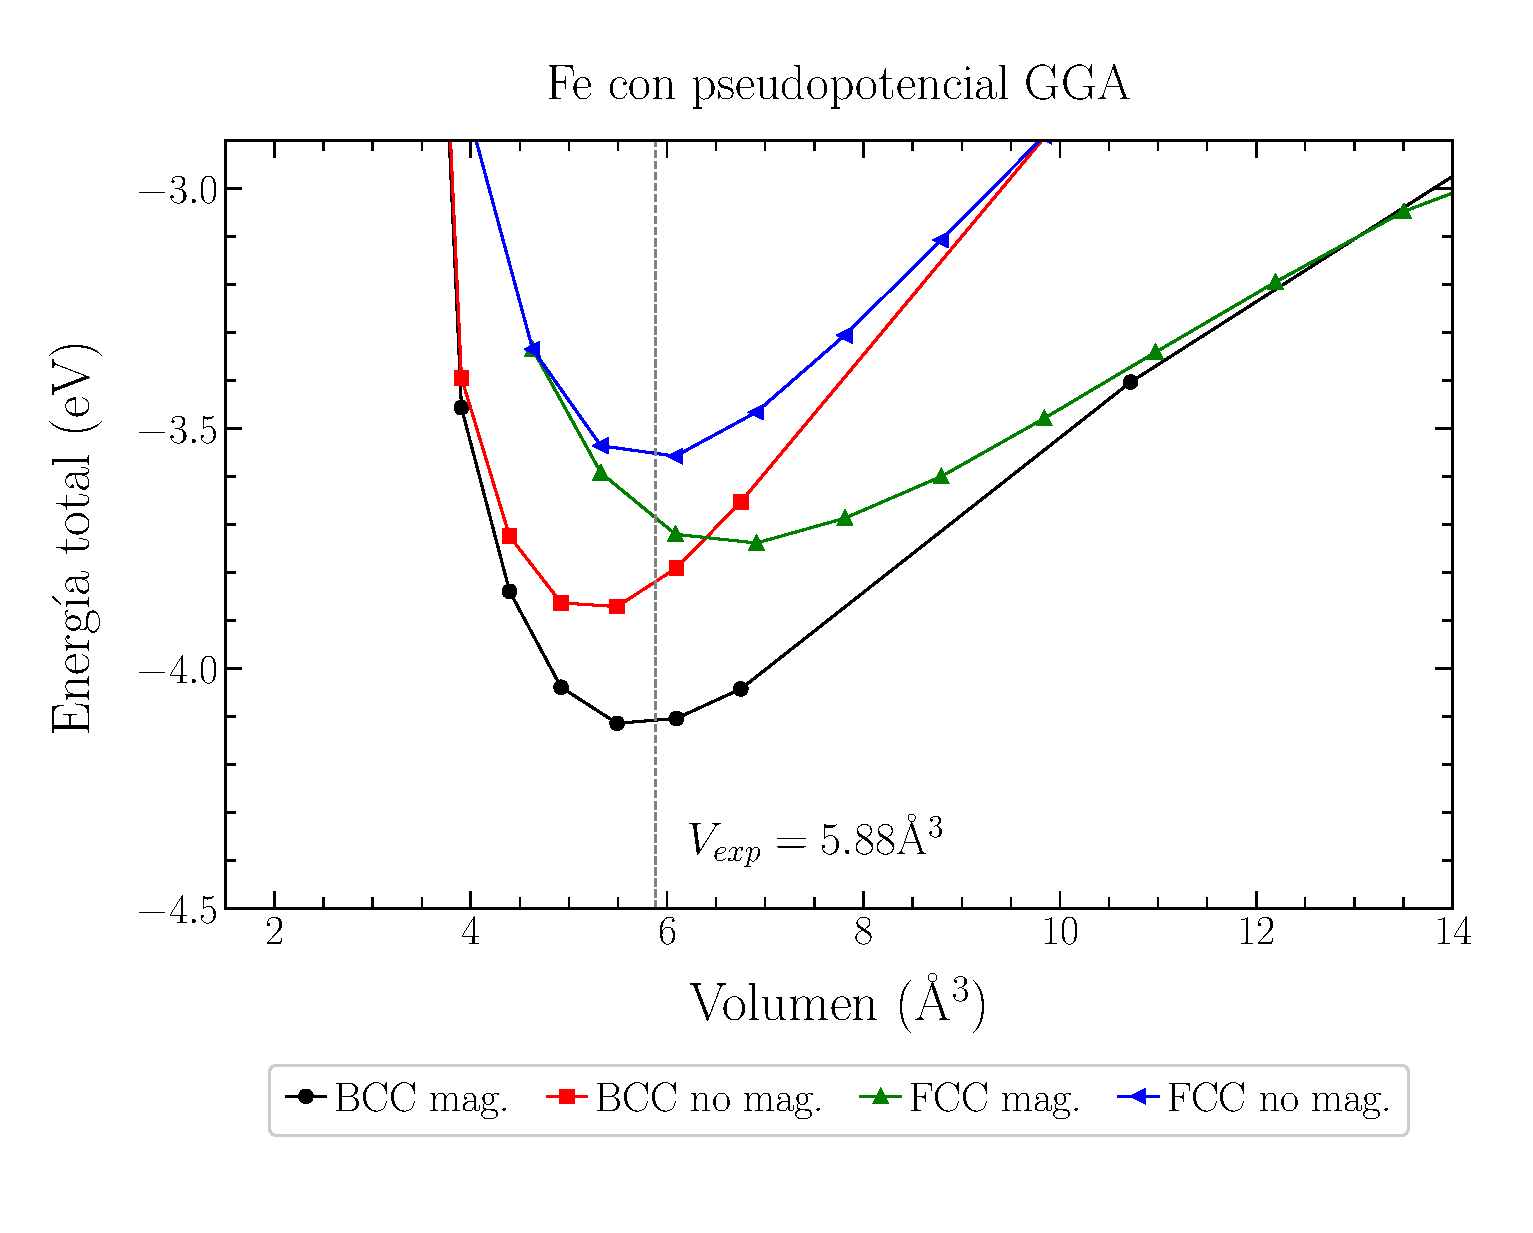
\includegraphics[width=0.6\textwidth]{Fe/punto5.eps}
\end{figure}

\vspace{0.5cm}
6. Resultados para Fe con estructura BCC y pseudopotenciales LDA:

\vspace{0.1cm}
(1) Caso magnético:

\begin{multicols}{2}
Convergencia en {\verb KPOINTS }:
\begin{verbatim}
K      Energía total 
4      -4.513904
6      -4.543464
8      -4.553608
10     -4.554087



\end{verbatim}

Convergencia en {\verb ENCUT }.
\begin{verbatim}
ENCUT  Energía total
240    -4.531648
270    -4.553569
300    -4.557551
330    -4.557006
360    -4.555172
380    -4.554126
400    -4.553608
\end{verbatim}
\end{multicols}

En la siguiente figura se comparan los resultados obtenidos del cálculo 
de Fe con estructura BCC utilizando los pseudopotenciales GGA (línea 
solida negra) y LDA (línea discontinua negra).
\begin{figure}[h]
\centering
 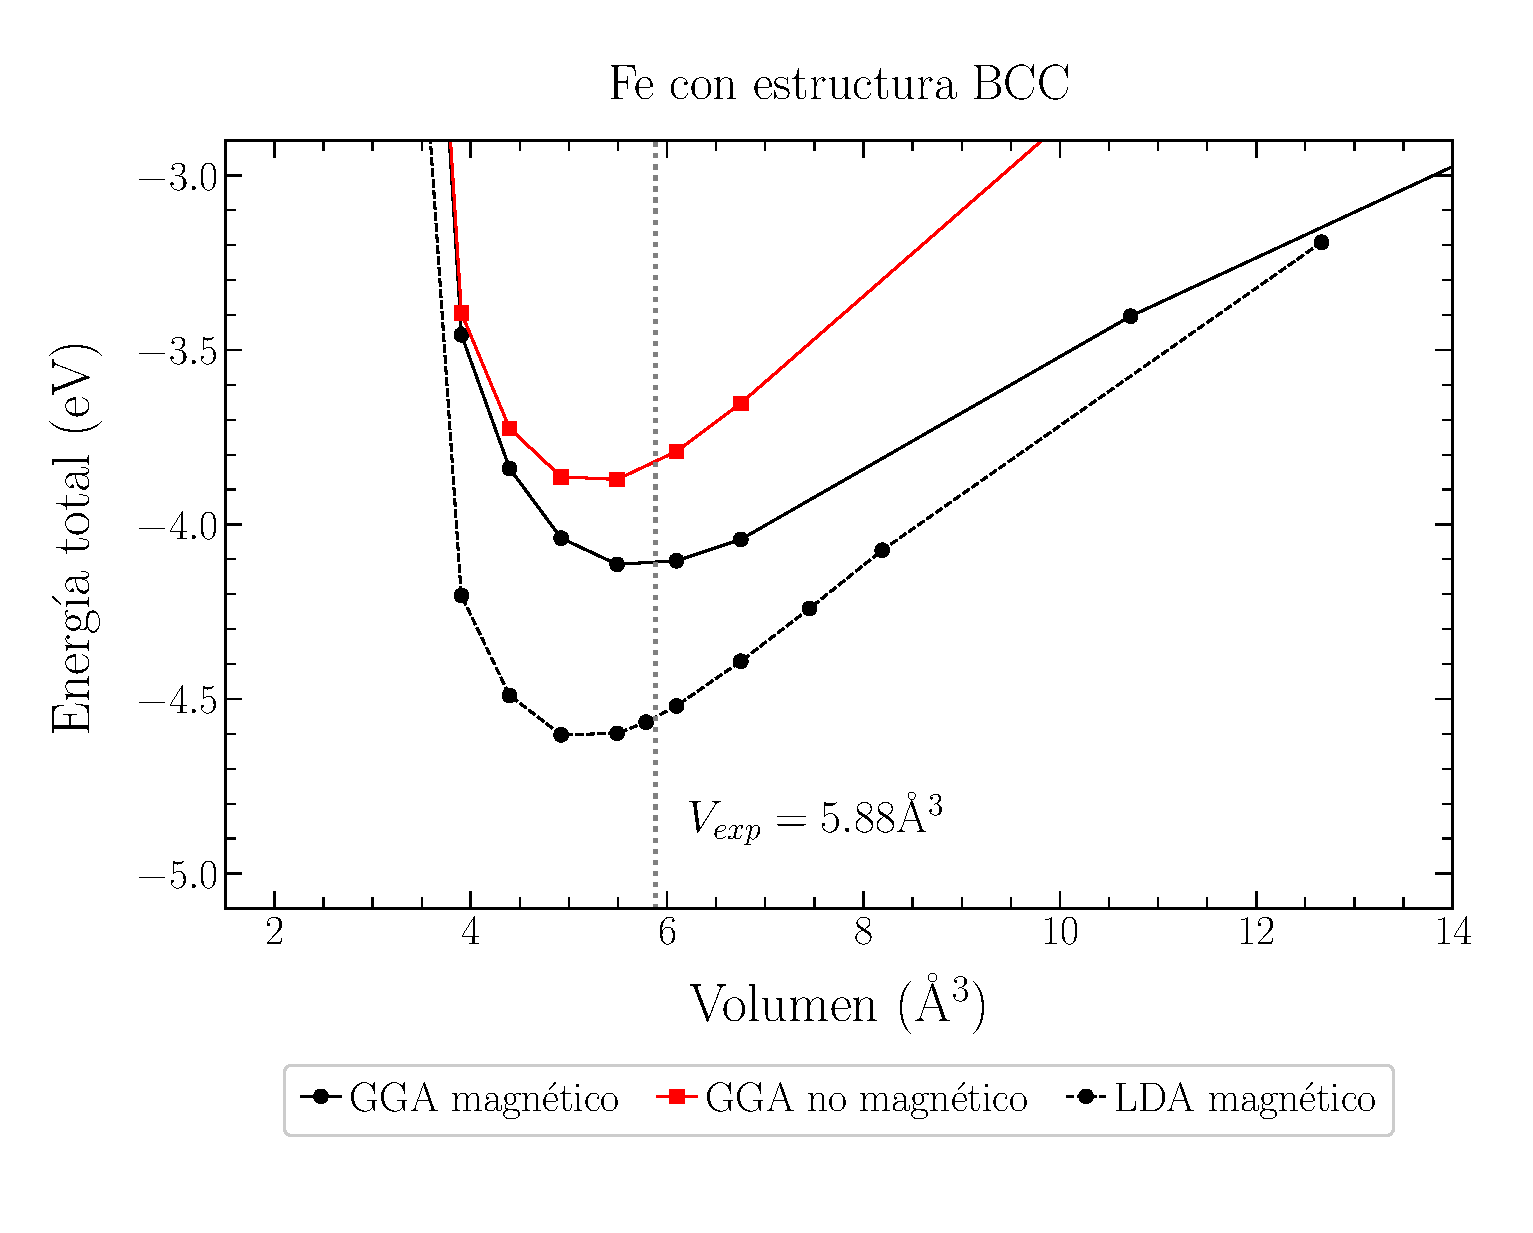
\includegraphics[width=0.6\textwidth]{Fe/punto6.eps}
\end{figure}

\newpage
7. Ajustamos la energía total en función del volumen del Fe-bcc con 
la ecuación de estado Birch--Murnaghan para los resultados obtenidos
con los pseudopotenciales GGA y LDA.
Nuevamente, implementando el paquete {\verb curve_fit } de 
{\verb scipy } integrado en python, los parámetros de ajuste 
encontrados fueron:
\begin{multicols}{2}
\begin{verbatim}
Parámetros de BCC GGA magnético:
E0 = -4.1136
B0 = 1.0410
V0 = 5.7612
B0' = 4.5862
\end{verbatim}

\begin{verbatim}
Parámetros de BCC LDA magnético:
E0 = -4.6005
B0 = 1.4034
V0 = 5.1892
B0' = 4.6272
\end{verbatim}
\end{multicols}

\begin{figure}[h]
\centering
 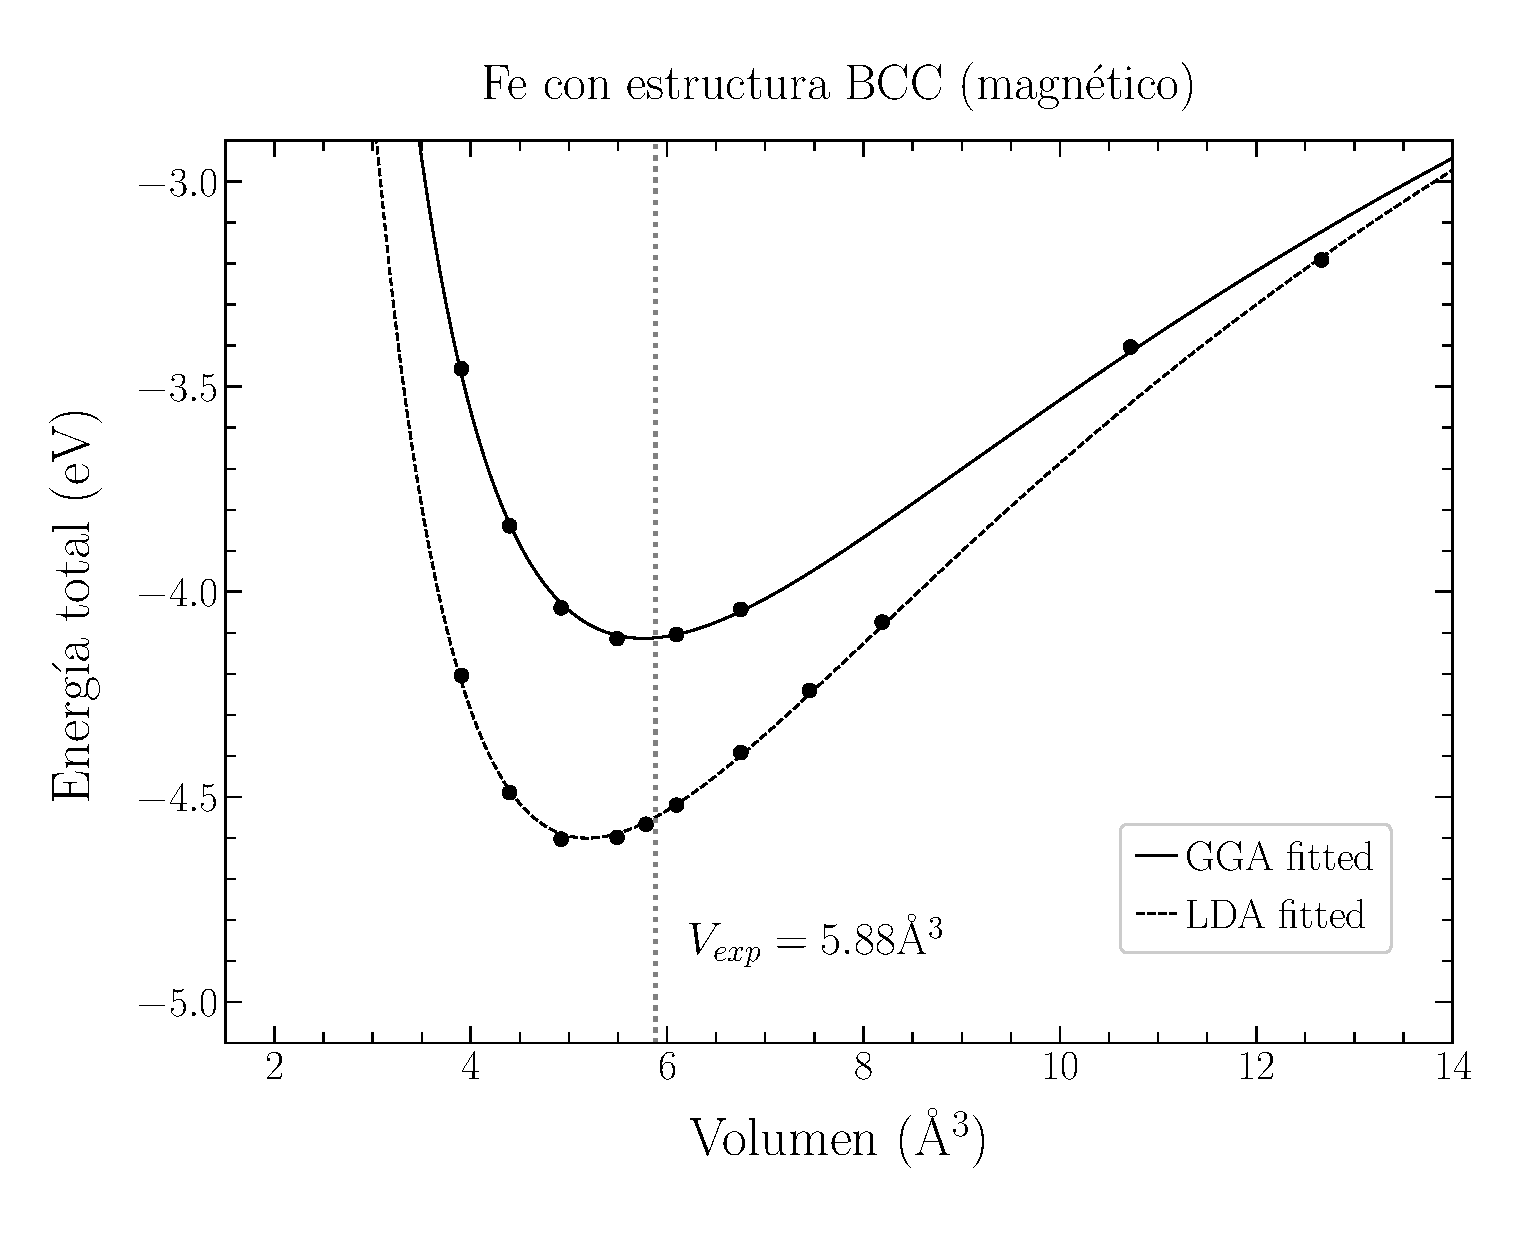
\includegraphics[width=0.55\textwidth]{Fe/punto7.eps}
\end{figure}

Calculando el parámetro de red a partir de los valores encontrados de
{\verb V0 }, tenemos:
\begin{verbatim}
a_GGA= 2.8457
a_LDA= 2.7482
\end{verbatim}
Por lo tanto, el cálculo que permite reproducir el valor experimental 
del parámetro de red ($a_{exp}=2.866$\AA) es el cálculo de estructura BCC con un pseudopotencial 
con correcciones de gradiente GGA.

\end{document}
